\begin{enumerate}
\item The maximum clock frequency in MHz of a 4-stage ripple counter, utilizing flip-flops, with each flip-flop having a propagation delay of 20 ns, is \rule{1cm}{0.10mm}. (round off to one decimal place)
\label{gate-ee-2022-29}
\hfill (GATE EE 2022)

\item The digital circuit shown \rule{1cm}{0.15mm}
\begin{center}
\begin{tikzpicture}
\ctikzset{                                   
logic ports=ieee,                   
logic ports/scale=0.5               
}                                    
\draw(-1.3,-0.56)node[nor port,anchor=out](x) {};  
%Drawing flip-flops
\draw (-1.3,-1.3) rectangle (0,0);
\draw(-1,-0.6) node{$D$};
\draw(-2,-1.1) node{$D_0$};
\draw(-0.2,-0.6) node{$Q$};
\draw(0.7,-1.3) rectangle (2,0);
\draw(1,-0.6) node{$D$};
\draw(1.8,-0.6) node{$Q$};
\draw(2.7,-1.3) rectangle (4,0);
\draw(3,-0.6) node{$D$};
\draw(3.8,-0.6) node{$Q$};
%connecting them
\draw(0,-0.6) -- (0.7,-0.6);
\draw(2,-0.6) -- (2.7,-0.6);
\draw(4,-0.6) -- (4.35,-0.6);
%drawing clk
\draw(-1.5,-2) node[above]{$CLK$} -- (3.35,-2);
%connecting clk 
\draw(-0.65,-2) -- (-0.65,-1.3);
\draw(1.35,-2) -- (1.35,-1.3);
\draw(3.35,-2) -- (3.35,-1.3);
\draw(3.35,-2) -- (4,-2);
%drawing clk edges
\draw(-0.5,-1.3) -- (-0.65,-1.1) -- (-0.8,-1.3);
\draw(1.2,-1.3) -- (1.35,-1.1) -- (1.5,-1.3);
\draw(3.2,-1.3) -- (3.35,-1.1) -- (3.5,-1.3);
%drawing Q2,Q1,Q0
%\draw(0.35,-0.6) --(0.35,0.2);
\draw(2.35,-0.6) --(2.35,0.3);
\draw(4.35,-0.6) --(4.35,0.9);
\draw(4.35,0.9) -- (-3,0.9);
\draw(2.35,0.3) -- (-2.5,0.3);
\draw(x.in 2) -|(-3,-0.7)to[short](-3,0.9);
\draw(x.in 1) -|(-2.5,-0.3)to[short](-2.5,0.3);
\draw(0.35,-0.3)node{$Q0$};
\draw(2.35,-0.35)node{$Q1$};
\draw(4.6,-0.35)node{$Q2$};
\end{tikzpicture}
\end{center}
\begin{enumerate}[label=(\Alph*)]
    \item is a divide-by-5 counter
    \item is a divide-by-7 counter
    \item is a divide-by-8 counter
    \item does not function as a counter due to disjoint cycles of states 
\end{enumerate}
\hfill{GATE IN 2022}
\item The propogation delay of the exclusive-OR(XOR) gate in the circuit in the figure is 3ns.The propogation delay of all the flip-flops is assumed to be zero.The clock(Clk) frequency provided to the circuit is 500MHz.
\label{prob:gate-ec-46.2021}
\hfill (GATE EC 2021)

\begin{tikzpicture}
\ctikzset{                                   
logic ports=ieee,                   
logic ports/scale=0.5               
}                                    
\draw(-1.3,-0.56)node[xor port,anchor=out](x) {};  
%Drawing flip-flops
\draw (-1.3,-1.3) rectangle (0,0);
\draw(-1,-0.6) node{$D2$};
\draw(0.7,-1.3) rectangle (2,0);
\draw(1,-0.6) node{$D1$};
\draw(2.7,-1.3) rectangle (4,0);
\draw(3,-0.6) node{$D0$};
%connecting them
\draw(0,-0.6) -- (0.7,-0.6);
\draw(2,-0.6) -- (2.7,-0.6);
\draw(4,-0.6) -- (4.35,-0.6);
%drawing clk
\draw(-1.5,-2) node[above]{$clk$} -- (3.35,-2);
%connecting clk 
\draw(-0.65,-2) -- (-0.65,-1.3);
\draw(1.35,-2) -- (1.35,-1.3);
\draw(3.35,-2) -- (3.35,-1.3);
%drawing clk edges
\draw(-0.5,-1.3) -- (-0.65,-1.1) -- (-0.8,-1.3);
\draw(1.2,-1.3) -- (1.35,-1.1) -- (1.5,-1.3);
\draw(3.2,-1.3) -- (3.35,-1.1) -- (3.5,-1.3);
%drawing Q2,Q1,Q0
\draw(0.35,-0.6) --(0.35,0.3);
\draw(2.35,-0.6) --(2.35,0.35);
\draw(4.35,-0.6) --(4.35,0.9);
\draw(4.35,0.9) -- (-3,0.9);
\draw(0.35,0.3) -- (-2.5,0.3);
\draw(x.in 2) -|(-3,-0.7)to[short](-3,0.9);
\draw(x.in 1) -|(-2.5,-0.3)to[short](-2.5,0.3);
\draw(0.35,0.5)node{$Q2$};
\draw(2.35,0.45)node{$Q1$};
\draw(4.35,1)node{$Q0$};
\end{tikzpicture}

Starting from the initial value of the flip-flop outputs $Q2Q1Q0 =111$ with $D2=1$,the minimum number of triggering clock edges after which the flip-flop outputs $Q2Q1Q0$ becomes 1 0 0\emph{(in integer)} is \line(1,0){12.5} 

\item  
\label{prob:gate IN 17}
For the $3$-bit binary counter shown in the figure, the output increments at every positive 
transition in the clock (CLK). Assume ideal diodes and the starting state of the counter as 
$000$. If output high is $1 V$ and output low is $0 V$, the current $I$(in mA) flowing through the 
$50 \Omega$ resistor during the $5$th clock cycle is (up to one decimal place)
\hfill(GATE IN 2018)
\begin{figure}[H]
\centering
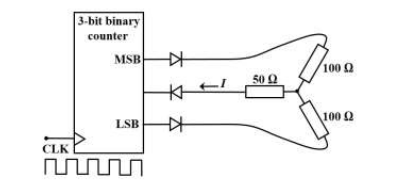
\includegraphics[width=\columnwidth]{ide/7474/figs/pic.png}
\caption{circuit}
\label{fig:lcd}
\end{figure}
\item
\label{prob:gate CS 22}
Consider the sequential circuit shown in the figure, where both flip-flops used are positive
    edge-triggered D flip-flops.
\begin{figure}[H]
        \centering      
        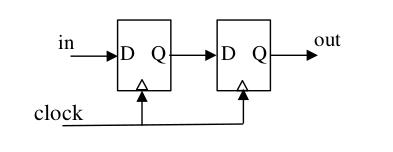
\includegraphics[width=\columnwidth]{ide/7474/figs/wert.jpg}
        \caption{ckt}    
        \label{fig:wert}
    \end{figure}

    \item The number of states in the state transition diagram of this circuit that have a transition back to the same state on some value of ''in'' is \rule{30pt}{1pt}.
   \hfill(GATE IN 2018)
   \item The synchronous sequential circuit shown below works at a clock frequency of $1 GHz$. The throughput, in $Mbits/s$,and the latency, in $ns$, respectively, are 
\begin{figure}[H]
    \centering
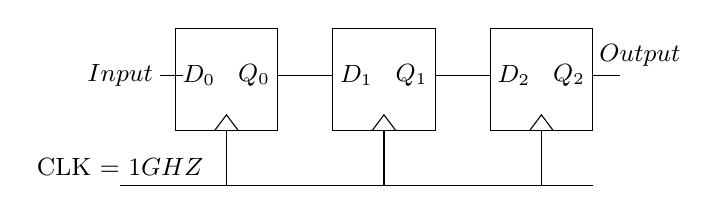
\begin{tikzpicture}
\ctikzset{                                  
    logic ports=ieee,                   
    logic ports/scale=0.5               
}                                    

% Drawing flip-flops
\draw (-1.3,-1.3) rectangle (0,0);
\draw(-1,-0.6) node{$D_0$};
\draw(-0.3,-0.6) node{$Q_0$};
\draw(0.7,-1.3) rectangle (2,0);
\draw(1,-0.6) node{$D_1$};
\draw(1.7,-0.6) node{$Q_1$};
\draw(2.7,-1.3) rectangle (4,0);
\draw(3,-0.6) node{$D_2$};
\draw(3.7,-0.6) node{$Q_2$};

% Connecting them
\draw(0,-0.6) -- (0.7,-0.6);
\draw(2,-0.6) -- (2.7,-0.6);
\draw(4,-0.6) -- (4.35,-0.6);
\draw(-1.2,-0.6) -- (-1.5,-0.6);

% Drawing clk
\draw(-2,-2) node[above]{CLK = $1GHZ$ } -- (3.35,-2);

% Connecting clk
\draw(-0.65,-2) -- (-0.65,-1.3);
\draw(1.35,-2) -- (1.35,-1.3);
\draw(3.35,-2) -- (3.35,-1.3);
\draw(3.35,-2) -- (4,-2);

% Drawing clk edges
\draw(-0.5,-1.3) -- (-0.65,-1.1) -- (-0.8,-1.3);
\draw(1.2,-1.3) -- (1.35,-1.1) -- (1.5,-1.3);
\draw(3.2,-1.3) -- (3.35,-1.1) -- (3.5,-1.3);

% Drawing Q2, Q1, Q0
\draw(0.35,-0.3)node{};
\draw(2.35,-0.35)node{};
\draw(4.6,-0.35)node{$ Output $};
\draw(-2,-0.6)node{$ Input $};
\end{tikzpicture}
\label{prob:gate EC 2023}
\end{figure}

    \begin{enumerate}
        \item $1000, 3$
         \item $333.33, 1$
          \item $2000, 3$
           \item $333.33 , 3$
    \end{enumerate}
\hfill(GATE EC 2023)
\label{prob:GATE EC 2023}
\item In a given sequential circuit, initial states are $Q1 = 1$ and $Q2 = 0$. For a clock frequency of $1 MHz$, the frequency of signal $Q2$ in kHz, is(rounded off to the nearest integer)
    
\begin{figure}[H]
    \centering
\begin{tikzpicture}              

%Drawing flip-flops
\draw (1.6,1.9) node {D Flip Flop};
\draw (0,0)--(3,0)--(3,4)--(0,4)--(0,0);
\draw(0.5,3.5) node{$D_1$};
\draw(2.5,3.5) node{$Q_1$};
\draw(2.5,0.5) node{$\bar{Q_1}$};
\draw(3.1,0.5) node{$\circ$};

\draw (8.6,1.9) node {D Flip Flop};
\draw(7,0)--(7,4)--(10,4)--(10,0)--(7,0);
\draw(7.5,3.5) node{$D_2$};
\draw(9.5,3.5) node{$Q_2$};
\draw(9.5,0.5) node{$\bar{Q_2}$};
\draw(10.1,0.5) node{$\circ$};

%connecting them
\draw(3.2,0.5)--(4.0,0.5);
\draw(10.2,0.5)--(10.9,0.5);
\draw(7.0,3.5)--(6.0,3.5);
\draw(4.0,0.5) -- (6.0,3.5);
\draw(10.0,3.5) -- (10.9,3.5);
\draw(4.0,3.5) --(3.0,3.5);

\draw(-1.1,-1.2)-- (8.5,-1.2);

%drawing clk
\draw (-1.0,-1.7)node{CLK =1Mhz};


%connecting clk 
\draw(1.5,-1.2) -- (1.5,0.0);
\draw(8.5,-1.2) -- (8.5,0.0);

%drawing clk edges
\draw(1.1,0.0) -- (1.48,0.4) -- (1.9,0.0);
\draw(8.1,0.0) -- (8.48,0.4) -- (8.9,0.0);

% Drawing Q2, D1,
\draw(10.9,3.5)--(10.9,5.4);
\draw(10.9,5.4)--(-1.0,5.4);
\draw(-1.0,5.4)--(-1.0,3.5);
\draw(0,3.5)--(-1.0,3.5);
\end{tikzpicture}
\end{figure}
\hfill(GATE EC 2023)

\item Neglecting the delays due to the logic gates in the circuit shown in figure, the 
decimal equivalent of the binary sequence $[ABCD]$ of initial logic states, which will not change with clock, is $\underline{\hspace{2cm}}$.\\

\hfill{(EE GATE 2023)}\\

\begin{figure}[H]
 \centering
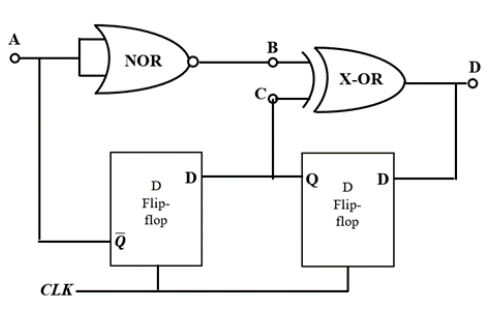
\includegraphics[width=\columnwidth]{ide/7474/figs/Gate_question.png}
\caption{Neglecting the delays}
\label{fig:Gate_question.png}
\end{figure}

\item 
Consider a sequential digital circuit consisting of T flip-flops and D flip-flops as shown in the figure. CLKIN is is the clock input to the circuit. At the beginning,Q1,Q2 and Q3 have values 0,1 and 1, respectively.
\hfill(GATE CS2023,43)

\begin{figure}[H]
\centering
\begin{circuitikz}
\tikzstyle{every node}=[font=\small]
\draw [short] (3.75,13.5) -- (3.75,11);
\draw [short] (3.75,11) -- (3.75,9.75);
\draw [short] (3.75,13.5) -- (6.25,13.5);
\draw [short] (6.25,13.5) -- (6.25,9.75);
\draw [short] (3.75,9.75) -- (6.25,9.75);
\draw [short] (12.5,13.5) -- (12.5,9.75);
\draw [short] (12.5,9.75) -- (15,9.75);
\draw [short] (15,9.75) -- (15,13.5);
\draw [short] (12.5,13.5) -- (15,13.5);
\draw [short] (3.75,12) -- (4,11.75);
\draw [short] (4,11.75) -- (3.75,11.5);
\draw [short] (12.5,12) -- (12.75,11.75);
\draw [short] (12.75,11.75) -- (12.5,11.5);
\draw[] (3.75,11.75) to[short] (1.25,11.75);
\draw [](6.25,13) to[short] (7.5,13);
\draw [](2.5,13) to[short] (3.75,13);
\draw [](3,10.5) to[short] (3.75,10.5);
\draw [](11.25,13) to[short] (12.5,13);
\draw [](11.5,10.25) to[short] (12.5,10.25);
\node [font=\small] at (4.25,13) {$J$};
\node [font=\small] at (4.25,10.5) {$K$};
\node [font=\small] at (5.75,13) {$Q$};
\node [font=\small] at (5.75,10.5) {$\overline{Q}$};
\node [font=\small] at (5,13.25) {SET};
\node [font=\small] at (5,10) {CLR};
\node [font=\small] at (8,13) {$Q_1$};
\node [font=\small] at (1.75,13) {$Q_{1}+Q_{2}$};
\node [font=\small] at (2,10.5) {$\overline{Q_1}+\overline{Q_2}$};
\draw[] (1.25,11.75) to[short] (0.75,11.75);
\draw [](0.75,11.75) to[short] (0.75,7.25);
\draw [](0.75,7.25) to[short] (1.5,7.25);
\draw [](0,7.25) to[short] (0.75,7.25);
\node [font=\small] at (-1,7.25) {Clock};
\node [font=\small] at (13,13) {$J$};
\node [font=\small] at (13,10.25) {$K$};
\node [font=\small] at (14.5,13) {$Q$};
\node [font=\small] at (14.5,10.25) {$\overline{Q}$};
\node [font=\small] at (13.75,13.25) {SET};
\node [font=\small] at (13.75,10) {CLR};
\node [font=\small] at (10,13) {$\overline{Q_1}+Q_2$};
\node [font=\small] at (10.25,10.25) {$Q_1+\overline{Q_2}$};
\draw (0,7.25) to[short] (0.75,7.25);
\draw [](15,13) to[short] (15.5,13);
\node [font=\small] at (15.75,13) {Q2};
\draw [](1.5,7.25) to[short] (8.5,7.25);
\draw [](8.5,7.25) to[short] (8.5,11.25);
\draw [](8.5,11.25) to[short] (8.5,11.5);
\draw[] (12.5,11.75) to[short] (8.5,11.75);
\draw [](8.5,11.75) to[short] (8.5,11.5);
\end{circuitikz}


\caption{Flip-Flop}
\label{fig:Flip-Flop}
\end{figure}
Which of the given values of \((Q_1, Q_2, Q_3)\) can NEVER be obtained with this digital circuit?
\begin{enumerate}
    
    \item ${(0,0,1)}$
    \item ${(1,0,0)}$
    \item ${(1,0,1)}$
    \item ${(1,1,1)}$
\end{enumerate}
\item In the circuit shift, the initial binary content of the shift register A $1101$ and that of shift register B is $1010$ The shift registers are positive edge triggered, and the gates have no delay.
when the shift control is high,what will be the binary content of the shift registers $A$ and $B$ after clock pulses?

\hfill{(GATE IN 2023)}

\begin{figure}[H]
\centering
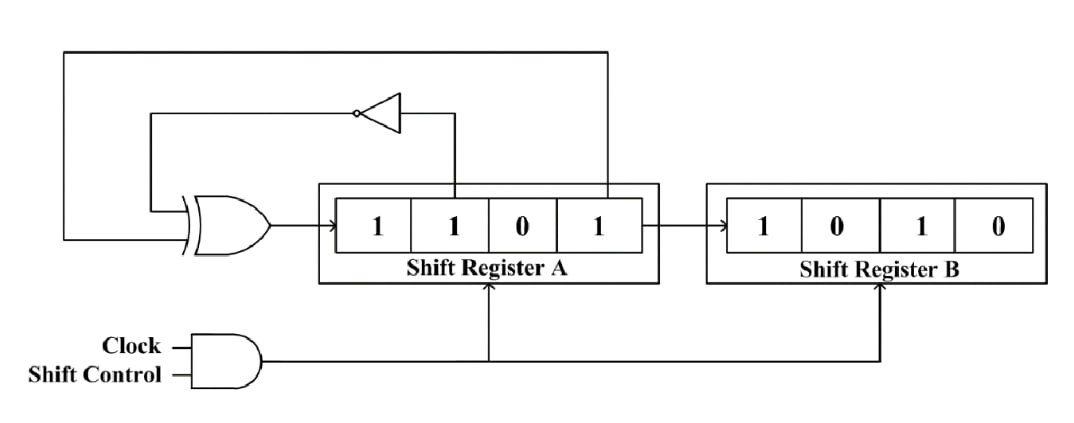
\includegraphics[width=\columnwidth]{ide/7474/figs/Gate.png}
\caption{circuit Digram}
\label{fig:cricuit Digram}
\end{figure}

\begin{enumerate}
\item $A= 1101,B=1101$
\item $A=1110 ,B=1001$
\item $A=0101 ,B=1101$
\item $A=1010 ,B=1111$
\end {enumerate}
\item For the circuit shown, the clock frequency is $f_0$ and the duty cycle is $25\%$. For the signal at the Q output of the Flip-Flop,\underline{\hspace{20pt}}.\hfill(GATE EC 2022)
		\begin{figure}[h]
			\centering
			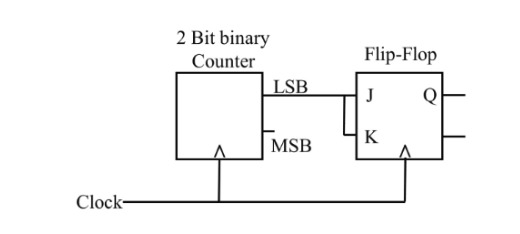
\includegraphics[width=\columnwidth]{ide/7474/figs/gate_image_new.jpg}
			\caption{Circuit}
			\label{fig:new_gate}
		\end{figure}
			\begin{enumerate}
			\item frequency is $\frac{{f_0}}{4}$ and duty cycle is $50\%$
			\item frequency is $\frac{{f_0}}{4}$ and duty cycle is $25\%$
			\item frequency is $\frac{{f_0}}{2}$ and duty cycle is $50\%$
			\item frequency is ${f_0}$ and duty cycle is $25\%$
		\end{enumerate}
\item In the circuit shown, the initial binary content of shift register A is 1101 and that of shift register B is 1010.The shift registers are positive edge triggered, and the gates have no delay.

When the shift control is high,what will be the binary content of the shift registers A and B after four clock pulses?
\hfill{(Gate IN 2023)}

		\begin{figure}[H]
			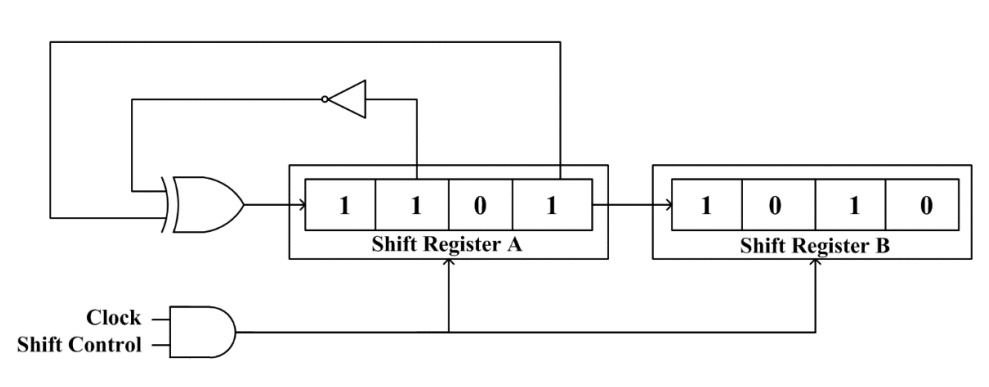
\includegraphics[width=\columnwidth]{figs/shift.jpeg}
			\caption{Shift register}
			\label{figs:fig1}
		\end{figure}
\begin{enumerate}
  \item A=1101,B=1101
  \item A=1110,B=1001
  \item A=0101,B=1101
  \item A=1010,B=1111
\end{enumerate}
\item The digital circuit shown in \figref{fig:GATEIN202236.png}
\begin{figure}[H]
  \centering
  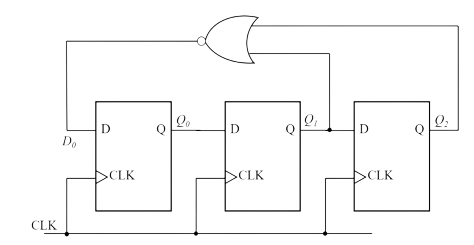
\includegraphics[width=\columnwidth]{ide/7474/figs/GATEIN202236.png}
  \caption{}
  \label{fig:GATEIN202236.png}
\end{figure}
 \begin{enumerate}
 \item is a divide-by-$5$ counter
 \item is a divide-by-$7$ counter
 \item is a divide-by-$8$ counter
 \item does not function as a counter due to disjoint cycles of states 
\end{enumerate}
\hfill(GATE-IN-2022)
\end{enumerate}
